\section{Etude de l'axe 3}
\subsection{Commande de la vitesse}

Nous allons maintenant déterminer la vitesse de sortie des vérins pour que la vitesse des points de la
 plate-forme soit constante.
 
 On propose le paramétrage suivant :
 \begin{itemize}
 \item le repère $\rep{0}=\repere{O_0}{x_0}{y_0}{z_0}$ est lié au châssis (0);
 \item le repère $\rep{5}=\repere{A}{x_5}{y_5}{z_0}$ est lié à l’ensemble \{berceau+parc échelle\} (5) 
 avec $\vect{O_0 A} = a\vy{0}$ et $\angl{x_0}{x_5} = \theta$, $\vect{AC}=c\vx{5}$ et $\vect{AD}= H\vx{5}$;
 \item le repère $\rep{3}=\repere{B}{x_3}{y_3}{z_3}$ est lié au châssis (3+4) 
  avec $\vect{O_0 B} = b\vx{0}$ et $\angl{x_0}{x_3} = \beta$, $\vect{BC}=r\vy{3}$.
  \end{itemize}

\begin{figure}[H]
\centering
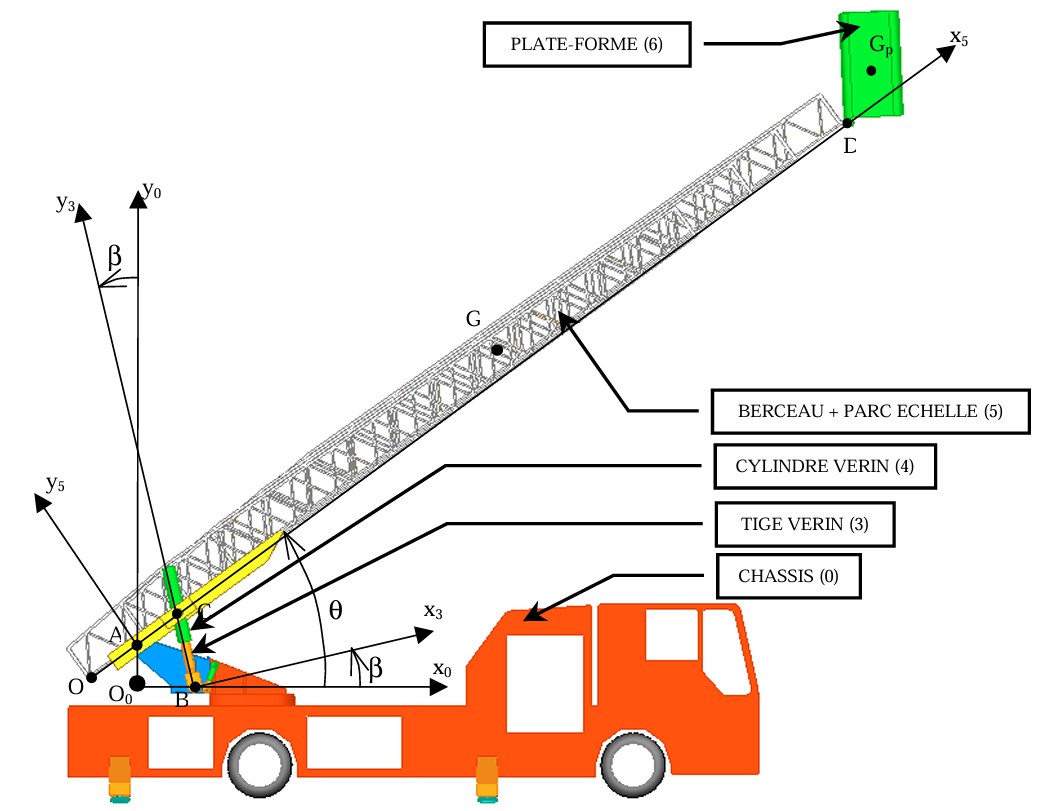
\includegraphics[width=.6\linewidth]{ccinp_psi_2007_fig_07}
\caption{\label{ccinp_psi_2007_fig_07} EPAS}
\end{figure}

%Q07
\question{Exprimer la vitesse du point $D$ du parc échelle dans son mouvement par rapport
 au châssis $\vectv{D}{5}{0}$ en fonction de la vitesse angulaire de dressage $\thetap$ et des paramètres
 géométriques.}
 \ifprof
 \begin{corrige}
 \end{corrige}
 \else
 \fi

%Q08
\question{ En faisant une fermeture de chaîne cinématique, déterminez la vitesse de sortie  du vérin 
$\vectv{C}{4}{3} = v\vy{3}$ en fonction de la vitesse angulaire de dressage et des paramètres géométriques.}
\ifprof
\begin{corrige}
\end{corrige}
\else
\fi

%Q09
\question{Etablir la relation $\tan \beta = \dfrac{b-c\cos\theta}{a+c\sin \theta}$ en écrivant une fermeture de chaîne géométrique.}
\ifprof
\begin{corrige}
\end{corrige}
\else
\fi

%Q10
\question{Déduire des questions précédentes la vitesse de sortie des vérins $v$ en fonction de
 $\theta$ et $H$ et des constantes $a$, $b$, $c$; pour que la vitesse du point $D $du parc échelle soit constante.}
\ifprof
\begin{corrige}
\end{corrige}
\else
\fi

\subsection{Dimensionnement des vérins}
 L’objet de cette partie est de déterminer la taille des vérins à utiliser dans cette chaîne fonctionnelle.
 On tiendra compte dans cette partie du fait que la plate-forme reste toujours horizontale.

\subsubsection{Géométrie du parc échelle}
Dans une première approche, on modélisera le parc échelle par un assemblage de trois plaques
 rectangulaires homogènes d’épaisseur négligeable, de longueur $L$ et de largeur $h$.
 Chaque plaque a une masse notée $m$.
 
 \begin{figure}[H]
\centering
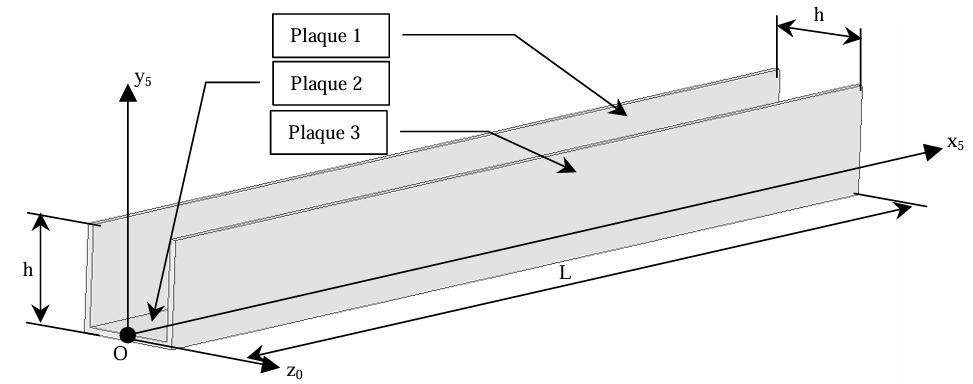
\includegraphics[width=.6\linewidth]{ccinp_psi_2007_fig_08}
\caption{\label{ccinp_psi_2007_fig_08} Géométrie du parc échelle}
\end{figure}



%Q11
\question{Montrez que le vecteur position $\vect{OG}$ du centre de gravité $G$ du parc échelle est
 tel que $\vect{OG}=\dfrac{L}{2}\vx{5}+\dfrac{h}{3}\vy{5}$.}
\ifprof
\begin{corrige}
\end{corrige}
\else
\fi

\subsubsection{Choix des vérins}
Les deux vérins doivent être capables de déplacer l’ensemble du parc échelle et la plate-forme
 chargée.


\begin{itemize}
\item Le parc échelle (5): on notera la matrice d’inertie du parc échelle au point $G$ (son centre de gravité) dans la base $\base{x_5}{y_5}{z_0}$ :  $\inertie{G}{5} = \matinertie{I_{Gx}}{I_{Gy}}{I_{Gz}}{0}{0}{0}{\base{x_5}{y_5}{z_0}}$. 
Le parc échelle a une masse notée $3m$ et une longueur notée $L$.
 Son centre de gravité $G$ est tel que $\vect{OG}=\dfrac{L}{2}\vect{x_5} +\dfrac{h}{3}\vect{y_5} $ .
 Le parc échelle est solidaire du berceau avec $\vect{OA}=d\vx{5}$.
 
\item La plate forme chargée (6) : pendant le redressement ou l’abaissement, la plate-forme reste toujours horizontale. Sa masse une fois chargée sera notée $M$ et son centre de gravité est le point $G_P$ tel que :
$\vect{DG_P} = \lambda \vx{0} + \mu \vy{0}$. On notera la matrice d’inertie de la plate forme chargée au point $G_P$ (son centre de gravité) dans la base $\base{x_0}{y_0}{z_0}$ : $\inertie{G_P}{6} = \matinertie{A}{B}{C}{0}{0}{0}{\base{x_0}{y_0}{z_0}}$.

\item  Le berceau (5): sa masse sera négligée devant les autres masses. Il est incliné par rapport à l’horizontal d’un angle $\theta$ fonction du temps.

\item Les vérins (3+4) : leurs masses seront négligées devant les autres masses.  Ils devront exercer un effort, modélisé par un glisseur de résultante $\vect{R}=R\vy{3}$ permettant le déplacement $\theta$.
 \end{itemize}

%Q12
\question{Déterminez l’expression littérale du moment dynamique en $A$ de l’ensemble \{parc échelle + berceau\} (5) par rapport au châssis (0) : $\vectmd{A}{5}{0}$.}
\ifprof
\begin{corrige}
\end{corrige}
\else
\fi


%Q13
\question{Déterminez l’expression littérale du moment dynamique en $A$ de la plate-forme (6) par rapport au châssis (0) : $\vectmd{A}{6}{0}$.}
\ifprof
\begin{corrige}
\end{corrige}
\else
\fi


%Q14
\question{Déterminez l’expression littérale de l’effort $R$ que devra  fournir l’ensemble des  deux vérins sur le berceau, en fonction des masses, des paramètres géométriques et de l’angle  $\theta$ et de ses dérivées. Indiquer clairement les sous-ensembles isolés, les actions mécaniques prises en compte et les théorèmes utilisés. }
\ifprof
\begin{corrige}
\end{corrige}
\else
\fi


%Q11
\question{}
\ifprof
\begin{corrige}
\end{corrige}
\else
\fi